\begin{activity} \label{A:11.8.4} Suppose the density of the cone defined by $r = 1 - z$, with $z \geq 0$, is given by $\delta(r, \theta, z) = z$. A picture of the cone is shown in Figure \ref{F:11.8.Cylindrical_ex}, and the projection of the cone onto the $xy$-plane in given in Figure \ref{F:11.8.Cylindrical_proj}.  Determine an iterated integral expression in cylindrical coordinates whose value is the mass of the cone.
\begin{figure}[ht]
\begin{center}
\begin{minipage}{2.5in}
\begin{center}
%\resizebox{!}{2.4in}{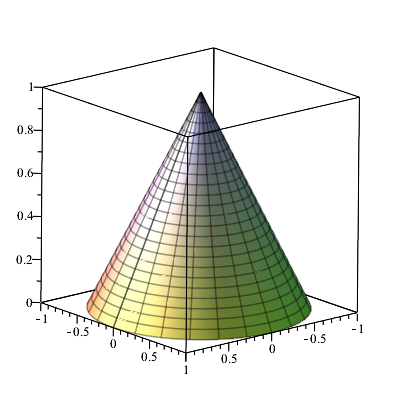
\includegraphics{11_8_Cylindrical_ex}}
  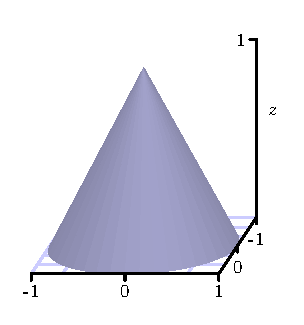
\includegraphics{figures/fig_11_8_cone.eps}
\end{center}
\caption{The cylindrical cone $r = 1-z$.}
\label{F:11.8.Cylindrical_ex}
\end{minipage} \hspace{0.5in}
\begin{minipage}{2.5in}
\begin{center}
%\resizebox{!}{2.4in}{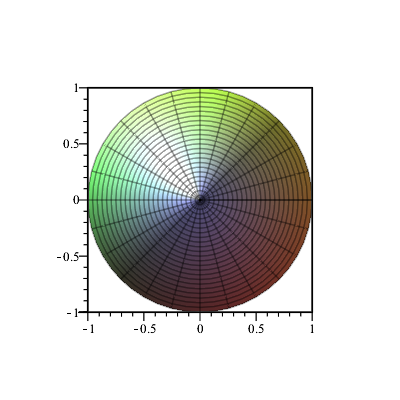
\includegraphics{11_8_Cylindrical_ex_proj}}
  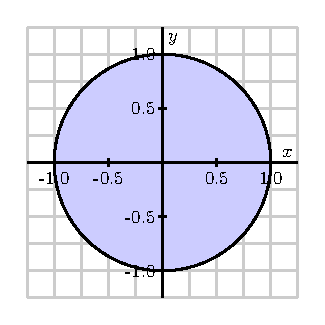
\includegraphics{figures/fig_11_8_cone_project.eps}
\end{center}
\caption{The projection into the $xy$-plane.}
\label{F:11.8.Cylindrical_proj}
\end{minipage}
\end{center}
\end{figure}



\end{activity}
\begin{smallhint}

\end{smallhint}
\begin{bighint}

\end{bighint}
\begin{activitySolution}
Recall that mass is the integral of density, so the mass of the cone is
\[\int \int \int_S \delta(r, \theta, z) \, dV.\]
The cone is bounded below by the $xy$-plane and above by the surface $r=1-z$. If we integrate with respect to $z$ first, then the limits on $z$ are $0 \leq z \leq 1-r$. When can project the surface into the $xy$-plane as shown in Figure \ref{F:11.8.Cylindrical_proj} to find the limits on $r$ and $\theta$. Note than when $z=0$ we have $r=1$, so the projection is a circle with radius centered at the origin. Therefore, the mass of the cone given the the iterated integral
\[\int \int \int_S \delta(r, \theta, z) \, dV = \int_0^{2\pi} \int_0^1 \int_0^{1-r} zr \, dz \, dr \, d\theta.\]
%\begin{align*}
%\int \int \int_S \delta(r, \theta, z) \, dV &= \int_0^{2\pi} \int_0^1 \int_0^{1-r} zr \, dz \, dr \, d\theta \\
%	&= \int_0^{2\pi} \int_0^1  r\frac{z^2}{2}\biggm|_0^{1-r} \, dr \, d\theta \\
%	&= \int_0^{2\pi} \int_0^1  r\frac{(1-r)^2}{2} \, dr \, d\theta \\
%	&= \int_0^{2\pi} \int_0^1  \frac{1}{2}\left(r - 2r^2 + r^3 \right) \, dr \, d\theta \\
%	&= \int_0^{2\pi}  \frac{1}{2}\left[\frac{r^2}{2} - \frac{2r^3}{3} + \frac{r^4}{4} \right]\biggm|_0^1  \, d\theta \\
%	&= \int_0^{2\pi}  \frac{1}{12}  \, d\theta \\
%	&= \frac{\pi}{6}.
%\end{align*}
\end{activitySolution}
\aftera
